\documentclass[10pt,onecolumn]{IEEEtran}

\usepackage[utf8]{inputenc}
\usepackage[T1]{fontenc}
\usepackage[spanish,es-tabla]{babel}
\usepackage{amsmath,amssymb}
\usepackage{graphicx}
\usepackage{booktabs}
\usepackage{array}
\usepackage{multirow}
\usepackage{float}
\usepackage{tikz}
\usetikzlibrary{positioning,arrows.meta,shapes.geometric,calc}
\usepackage{circuitikz}
\usepackage{hyperref}
\usepackage{siunitx}
\usepackage{caption}

\renewcommand{\abstractname}{Resumen}

\title{Diseño e Implementación de un Semáforo Vehicular y Peatonal 
Basado en Lógica Digital Discreta\\ 
\large Propuesta de Diseño}

\author{
\IEEEauthorblockN{1\textsuperscript{st} Kevin Méndez Carvajal}
\IEEEauthorblockA{
    \textit{Ingeniería en Electrónica} \\
    \textit{Instituto Tecnológico de Costa Rica} \\
    Laboratorio de Electrónica Analógica \\
    kemendez@estudiantec.cr
}
\\
\and
\IEEEauthorblockN{2\textsuperscript{nd} Brandon Nájera Zúñiga}
\IEEEauthorblockA{
    \textit{Ingeniería en Electrónica} \\
    \textit{Instituto Tecnológico de Costa Rica} \\
    Laboratorio de Electrónica Analógica \\
    brandonnz@estudiantec.cr
}
\\
\and
\IEEEauthorblockN{3\textsuperscript{rd} Wilson Osejo Ruiz}
\IEEEauthorblockA{
    \textit{Ingeniería en Electrónica} \\
    \textit{Instituto Tecnológico de Costa Rica} \\
    Laboratorio de Electrónica Analógica \\
    wilsonruiz@estudiantec.cr
}
}

\begin{document}
\maketitle

\begin{abstract}
El presente documento describe la propuesta de diseño de un sistema de semáforo vehicular y peatonal implementado en su totalidad con electrónica digital discreta, sin el empleo de microcontroladores ni dispositivos lógicos programables. El sistema se organiza en tres subsistemas funcionales: (i) una fuente de alimentación lineal que transforma la red de \SI{120}{\volt_{AC}} en niveles de continua regulados; (ii) una unidad de control lógico secuencial encargada de gestionar los tiempos del ciclo semafórico, un display de siete segmentos para la cuenta regresiva peatonal y un generador de audio para la señalización sonora; y (iii) un subsistema de iluminación de potencia que conmuta los arreglos de diodos emisores de luz (LED) vehiculares y peatonales. Se presenta el diagrama de bloques general, la máquina de estados que rige la secuencia de luces, los criterios de selección de componentes y los lineamientos para la simulación en Multisim y la posterior implementación física en al menos dos placas de circuito impreso (PCB).
\end{abstract}

\renewcommand{\IEEEkeywordsname}{Palabras Clave}
\begin{IEEEkeywords}
Semáforo, lógica secuencial, temporizador 555, contador BCD, decodificador de siete segmentos, fuente lineal, regulador de voltaje, driver de LED, PCB.
\end{IEEEkeywords}


% 1. INTRODUCCIÓN

\section{Introducción}
La regulación del tránsito vehicular y peatonal en intersecciones urbanas constituye uno de los problemas de ingeniería de control más representativos para la enseñanza de la electrónica digital, dado que combina temporización precisa, lógica secuencial, interfaces de potencia y, en su versión completa, la integración de subsistemas analógicos (fuente de alimentación, amplificación de audio) con subsistemas digitales (contadores, decodificadores, máquinas de estado). El presente proyecto retoma este problema clásico con la restricción pedagógica de prescindir de cualquier dispositivo programable —microcontroladores, FPGA o plataformas tipo Arduino—, forzando la solución hacia la integración de circuitos integrados de mediana escala (MSI) tales como contadores síncronos, decodificadores BCD a siete segmentos, temporizadores 555 y biestables discretos.

Desde la perspectiva de la integración análogo-digital, el proyecto exige que el diseñador resuelva simultáneamente tres dominios de diseño que en la práctica profesional rara vez se abordan de forma aislada: el diseño de fuentes de alimentación lineales con disipación térmica calculada (dominio analógico de potencia), el diseño de máquinas de estado y bases de tiempo digitales (dominio digital secuencial), y el diseño de etapas de conmutación e interfaz de potencia para cargas de alto consumo como arreglos de LED (dominio de electrónica de potencia a pequeña escala). Esta propuesta de diseño documenta el análisis preliminar de los tres subsistemas, sienta las bases topológicas y conceptuales de cada etapa, y deja explícitamente señalados los puntos en los que se requieren los valores numéricos definitivos (tiempos de ciclo, referencias de circuitos integrados disponibles en laboratorio y parámetros del oscilador de audio) que serán proporcionados en una iteración posterior del proyecto.


% 2. OBJETIVOS

\subsection{Objetivo General}
Introducir aprendizaje de ingeniería en donde requiera poner en práctica las habilidades y conceptos adquiridos en el uso de las herramientas de simulación, equipos de medición y prototipado.

\subsection{Objetivos Específicos}
\begin{enumerate}
    \item Diseñar una fuente de alimentación lineal completa (transformador, rectificador, filtro y reguladores) capaz de suministrar las tensiones necesarias al sistema, con el adecuado manejo de disipación térmica.
    \item Implementar la lógica secuencial de control del semáforo utilizando exclusivamente circuitos integrados digitales discretos (temporizadores, contadores, compuertas y biestables), sin dispositivos programables, para gestionar los tiempos de 30~s, 5~s y 20~s, así como la cuenta regresiva en displays de 7 segmentos y la señal de audio con cambio de frecuencia.
    \item Diseñar los circuitos de conmutación (drivers transistorizados) para el manejo de los arreglos de LEDs vehiculares y peatonales, asegurando la correcta iluminación y la disipación de potencia.
    \item Utilizar herramientas de simulación (Multisim, Circuit Wizard) para verificar la integración de las tres etapas (alimentación, control y potencia), y posteriormente implementar el sistema completo en una maqueta física con al menos dos circuitos impresos fabricados en laboratorio.
    \item Fomentar el trabajo colaborativo en equipo, aplicando buenas prácticas de ensamblaje, medición y documentación técnica bajo el formato IEEE y control de versiones.
\end{enumerate}


% 3. DIAGRAMA DE BLOQUES GENERAL

\section{Diagrama de Bloques General}
\label{sec:bloques}

El sistema se concibe como la interconexión jerárquica de tres subsistemas principales. El subsistema de alimentación entrega los niveles de tensión regulados necesarios tanto a la lógica de control (nivel TTL/CMOS) como a las etapas de potencia del subsistema de iluminación; el subsistema de control lógico genera las señales de habilitación, los códigos BCD de cuenta regresiva y la señal de audio, mientras que el subsistema de iluminación recibe dichas señales lógicas y las traduce en corrientes de conmutación capaces de excitar los arreglos de LED. La Fig.~\ref{fig:bloques} resume dicha jerarquía.

\begin{figure}[H]
\centering
\begin{tikzpicture}[
    block/.style={draw, rectangle, rounded corners, minimum width=3.1cm, minimum height=1.1cm, align=center, font=\small},
    sub/.style={draw, rectangle, dashed, inner sep=8pt},
    arrow/.style={-{Latex[length=2mm]}, thick}
]
% Subsistema 1: Fuente
\node[block] (fuente) {Subsistema 1\\Fuente de Alimentación\\120 VAC $\to$ DC regulado};

% Subsistema 2: Control
\node[block, below=1.4cm of fuente, xshift=-3.4cm] (control) {Subsistema 2\\Control Lógico Secuencial};
\node[block, below=0.6cm of control] (display) {Display 7 Seg.\\(BCD/Decodificador)};
\node[block, below=0.6cm of display] (audio) {Generador y\\Amplificador de Audio};

% Subsistema 3: Iluminación
\node[block, below=1.4cm of fuente, xshift=3.4cm] (driver) {Subsistema 3\\Drivers de Conmutación};
\node[block, below=0.6cm of driver] (leds) {Arreglos LED\\Vehicular / Peatonal};

% Entrada
\node[block, above=0.9cm of fuente, fill=gray!10] (red) {Red Eléctrica\\120 VAC, 60 Hz};

% Entrada peatonal
\node[block, left=1.0cm of control, fill=gray!10] (boton) {Pulsador de\\Solicitud Peatonal};

% Conexiones
\draw[arrow] (red) -- (fuente);
\draw[arrow] (fuente.south) -- ++(0,-0.35) -| (control.north);
\draw[arrow] (fuente.south) -- ++(0,-0.35) -| (driver.north);
\draw[arrow] (control) -- (display);
\draw[arrow] (control) -- (audio);
\draw[arrow] (control.east) -- (driver.west) node[midway, above, font=\tiny]{señales lógicas};
\draw[arrow] (driver) -- (leds);
\draw[arrow] (boton) -- (control);

\end{tikzpicture}
\caption{Diagrama de bloques general del sistema y su jerarquía de subsistemas.}
\label{fig:bloques}
\end{figure}


% 4. DESARROLLO TÉCNICO

\section{Desarrollo Técnico}

% ----------------------------------------------------------
\subsection{Subsistema 1: Alimentación (AC/DC)}
\label{subsec:fuente}

El subsistema de alimentación convierte la tensión de red de \SI{120}{\volt_{AC}} a \SI{5}{\volt_{DC}} regulado para alimentar la lógica digital del semáforo. La implementación utiliza un transformador con rectificación de onda completa mediante un puente de diodos.

\subsubsection{Descripción del circuito implementado}

Se parte de la red eléctrica de \SI{120}{\volt_{AC}}, \SI{60}{\hertz}. El transformador MIYAKO LP-573 (relación 10:1) reduce la tensión, obteniendo aproximadamente \SI{12}{\volt_{AC}} en el secundario. Posteriormente, se realiza una rectificación de onda completa mediante un puente de diodos 1N4007, se filtra con un capacitor electrolítico de \SI{4700}{\micro\farad} a \SI{25}{\volt}, y finalmente se regula con un LM7805 provisto de disipador de calor. Antes de ingresar al regulador se coloca una resistencia de \SI{50}{\ohm} / \SI{5}{\watt} en serie para limitar las corrientes de arranque. A la salida del LM7805 se colocan dos capacitores en paralelo: \SI{0.1}{\micro\farad} (cerámico, para alta frecuencia) y \SI{10}{\micro\farad} (electrolítico, para baja frecuencia), de cuyo nodo se extraen los \SI{+5}{\volt} que alimentan el resto del circuito.

Las características principales de los componentes son:
\begin{itemize}
    \item \textbf{Transformador MIYAKO LP-573}: Relación 10:1, salida nominal \SI{12}{V_{AC}}.
    \item \textbf{Diodo 1N4007}: Rectificador de silicio, $V_{RRM}=\SI{1000}{V}$, $I_{F(AV)}=\SI{1}{A}$, caída directa $\approx \SI{0.7}{V}$.
    \item \textbf{Capacitor de filtro}: \SI{4700}{\micro\farad} / \SI{25}{V}.
    \item \textbf{Regulador de voltaje}: LM7805 con disipador térmico.
    \item \textbf{Resistencia de limitación}: \SI{50}{\ohm} / \SI{5}{W} en serie antes del regulador.
    \item \textbf{Resistencia de carga de prueba}: \SI{50}{\ohm} / \SI{5}{W}.
\end{itemize}

\subsubsection{Reguladores lineales y justificación}

En la implementación real del sistema se utiliza únicamente el regulador lineal LM7805, el cual entrega \SI{5}{\volt_{DC}} regulados para alimentar toda la lógica digital del semáforo (contadores, decodificador BCD a 7 segmentos, máquina de estados, oscilador de audio, etc.). Aunque la propuesta inicial contemplaba el uso de reguladores adicionales para los arreglos de LED, en esta etapa se trabaja con un único nivel de \SI{5}{\volt} para simplificar el diseño y reducir el número de componentes.

\subsubsection{Cálculo de disipación de calor}

La potencia disipada en el regulador LM7805 se calcula con la ecuación:

\begin{equation}
P_D = (V_{IN} - V_{OUT}) \cdot I_L
\label{eq:potencia_disipada}
\end{equation}

Donde $V_{OUT} = \SI{5}{\volt}$, $V_{IN} \approx \SI{15}{\volt}$ (voltaje aproximado después del puente rectificador y el capacitor de filtro de \SI{4700}{\micro\farad}), e $I_L \approx \SI{100}{\milli\ampere}$ (corriente con la resistencia de carga de \SI{50}{\ohm}):

\begin{equation}
P_D = (15 - 5) \times 0.1 = \SI{1.0}{\watt}
\end{equation}

La temperatura de juntura se estima mediante:

\begin{equation}
T_J = T_A + P_D \cdot \theta_{JA}
\label{eq:temp_juntura}
\end{equation}

Con el LM7805 provisto de disipador, se estima $\theta_{JA} \approx \SI{22}{\celsius\per\watt}$:

\[
\Delta T = 1.0 \times 22 = \SI{22}{\celsius} \quad \Rightarrow \quad T_J \approx \SI{47}{\celsius}
\]

Este valor está muy por debajo del límite máximo del fabricante (\SI{125}{\celsius}), confirmando que el regulador opera en condiciones térmicas seguras.

\subsubsection{Esquemático de la fuente}
\begin{figure}[H]
\centering
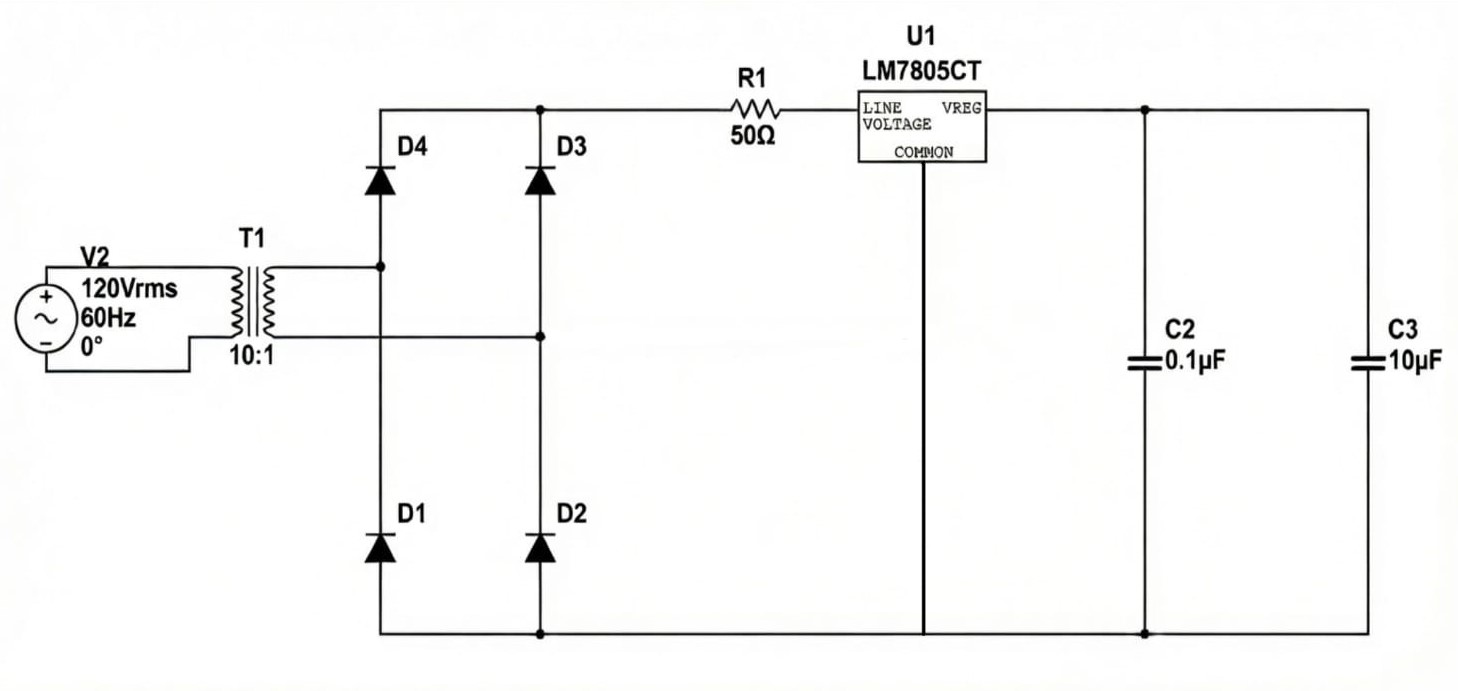
\includegraphics[width=0.85\textwidth]{fuente}
\caption{Esquemático completo del subsistema de alimentación.}
\label{fig:fuente}
\end{figure}

\subsubsection{Implementación física del PCB}

La implementación en protoboard del sistema completo se llevó a cabo con los componentes disponibles en la bodega del laboratorio, complementados con adquisiciones propias del equipo en establecimientos comerciales locales. Esta combinación de fuentes de suministro implicó en algunos casos trabajar con versiones o fabricantes alternativos de un mismo integrado, todos ellos funcionalmente equivalentes y compatibles con los niveles lógicos TTL/CMOS de \SI{5}{\volt} del sistema. El cableado interno de las protoboards se realizó con cables de protoboard estándar, resultando en un conexionado funcional aunque visualmente denso dado el alto número de interconexiones entre integrados. Para la vinculación de las protoboards con la maqueta se utilizaron cables de conexión que permitieron enlazar los LEDs de los postes y los displays de 7 segmentos sin requerir soldadura directa sobre la estructura, decisión motivada principalmente por las restricciones de tiempo del proyecto.

El diseño del circuito impreso fue elaborado en Eagle CAD previo al envío a fabricación externa, lo que permitió verificar la correcta asignación de huellas, la continuidad de las redes eléctricas y la viabilidad del ruteo antes de comprometer el diseño a fabricación, reduciendo el riesgo de errores en el PCB físico. Las Figs.~\ref{fig:pcb_antes} y~\ref{fig:pcb_despues} muestran el resultado del circuito impreso del subsistema de alimentación antes y después del proceso de soldadura de componentes.

\begin{figure}[H]
\centering
\begin{minipage}{0.48\columnwidth}
    \centering
    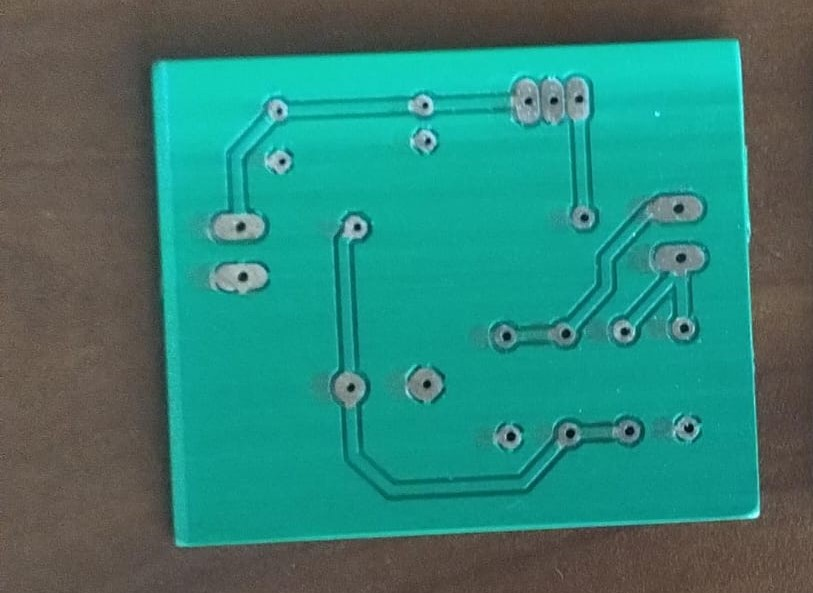
\includegraphics[width=\linewidth]{pcb1}
    \caption{PCB de la fuente de alimentación antes de soldar.}
    \label{fig:pcb_antes}
\end{minipage}\hfill
\begin{minipage}{0.48\columnwidth}
    \centering
    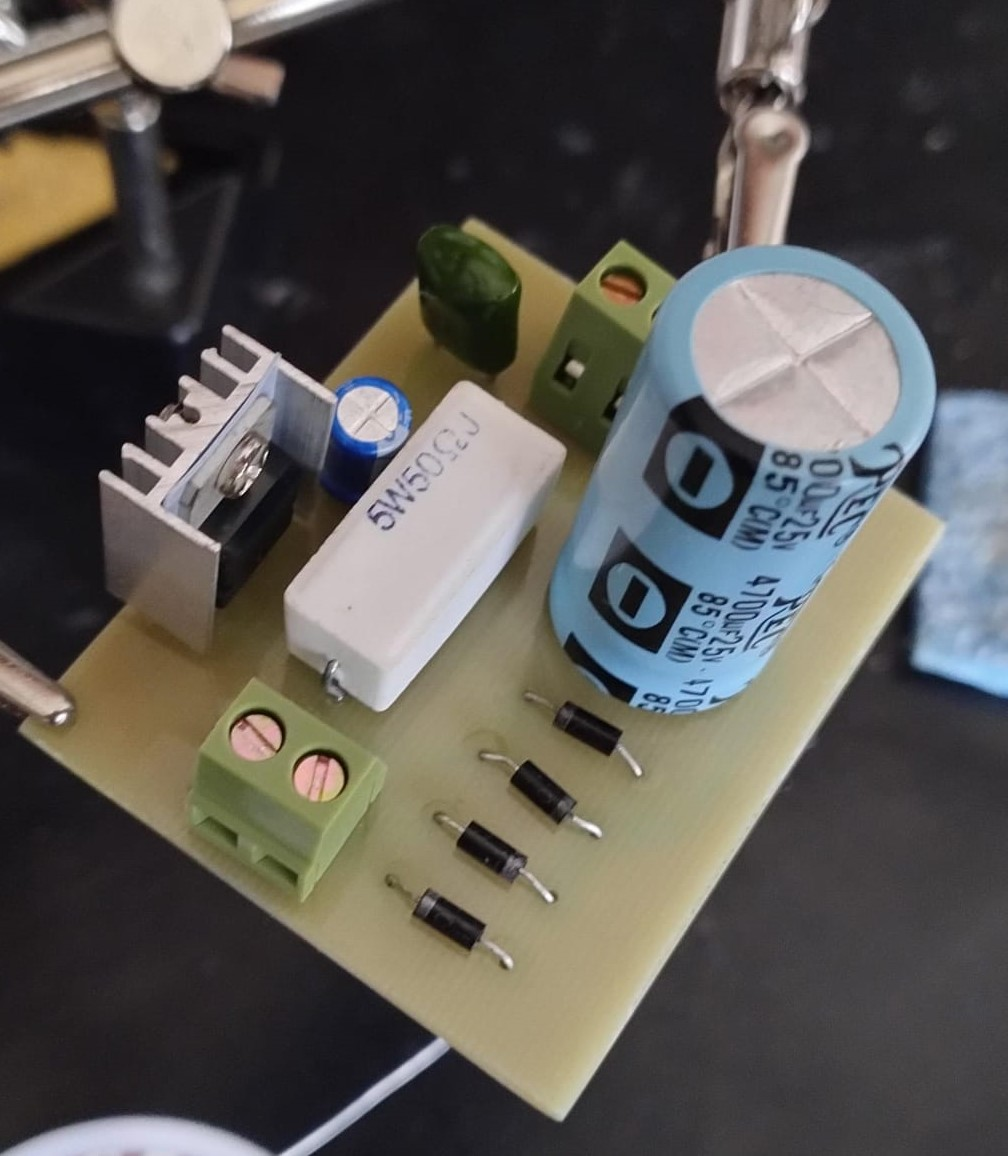
\includegraphics[width=\linewidth]{pcb2}
    \caption{PCB de la fuente de alimentación después de soldar.}
    \label{fig:pcb_despues}
\end{minipage}
\end{figure}

% ----------------------------------------------------------
\subsection{Subsistema 2: Control Lógico, Display y Sonido}
\label{subsec:control}

Este subsistema constituye el núcleo de decisión del semáforo y fue implementado exclusivamente con lógica combinacional y secuencial discreta, utilizando circuitos integrados de mediana escala (MSI) sin ningún dispositivo programable.

\subsubsection{Bases de tiempo (temporizadores maestros)}

La referencia temporal del sistema se genera mediante tres temporizadores LM555CM configurados en modo astable. El primero produce la base de tiempo principal de conteo (reloj de \SI{1}{\hertz}); el segundo genera el tono de audio normal durante la fase de cruce peatonal; y el tercero produce el tono agudo de aviso en los últimos 5 segundos.

La frecuencia de oscilación de cada temporizador sigue la ecuación:

\begin{equation}
f_{osc} = \frac{1.44}{(R_1 + 2R_2)\,C_1}
\label{eq:555_astable}
\end{equation}

Para la base de tiempo de \SI{1}{\hertz} se utilizaron $R_1 = \SI{33}{\kilo\ohm}$, $R_2 = \SI{56}{\kilo\ohm}$ y $C_1 = \SI{10}{\micro\farad}$, con un capacitor de \SI{10}{\nano\farad} en el pin CON para estabilidad. El pin TRI del temporizador de reloj se conecta al nodo entre $R_2$ y $C_1$ (pines DIS, THR y TRI unidos en dicho nodo), y su salida (OUT) va directamente al pin DOWN del contador de unidades 74LS192N, proporcionando los pulsos de decremento de un segundo.

Para el control del semáforo vehicular se emplean dos temporizadores adicionales: uno configurado con \SI{50}{\kilo\ohm} y \SI{100}{\micro\farad} para la fase amarilla (~3 segundos), cuya salida activa mediante transistor Q1 (2N2222A) el LED amarillo vehicular y alimenta una entrada de la compuerta 74ALS02N; y otro con \SI{250}{\kilo\ohm} y \SI{100}{\micro\farad} para la fase roja vehicular y verde peatonal. Para la señalización sonora se utilizan dos temporizadores adicionales (Temporizadores 4 y 5) que, en conjunto, producen tonos audibles de alerta durante el cambio de fase peatonal.

\subsubsection{Sistema de conteo y display de cuenta regresiva}

El tiempo de cruce peatonal de \SI{25}{\second} se implementa con dos contadores síncronos 74LS192N en cascada (unidades y decenas) operando en modo descendente, partiendo del valor 25 y decrementando hasta 0. Los preajustes de carga se fijan en binario: unidades en 0101 ($A=V_{CC}$, $B=GND$, $C=V_{CC}$, $D=GND$, es decir, valor 5) y decenas en 0010 ($B=V_{CC}$, resto a GND, es decir, valor 2). El pin LOAD de ambos contadores, junto con el CLR del flip-flop 74LS74D, se conecta a un nodo común con una resistencia de \SI{10}{\kilo\ohm} a $V_{CC}$ y un pulsador a masa para reinicio manual. El pin Borrow Out (BO) del contador de unidades alimenta el pin DOWN del contador de decenas, de modo que al llegar a 0 en las unidades se decrementa la decena.

La salida BCD de cada contador se decodifica mediante un integrado 4511BD (decodificador BCD a 7 segmentos con latch interno), con los pines $\overline{EL}$ a masa y $\overline{BI}$, $\overline{LT}$ a $V_{CC}$. Cada segmento del display se protege con resistencias limitadoras de \SI{330}{\ohm}.

La detección del estado de cuenta cero se implementa mediante lógica combinacional: una compuerta NOR de 4 entradas (que recibe QA, QB, QC y QD del contador de decenas) cuya salida es 1 únicamente cuando todas las salidas son 0, combinada con un arreglo de inversores 7404N y compuertas AND 7408J para detectar el estado cero del contador de unidades. La salida de este arreglo, unida mediante una compuerta 7408J, activa el pin 1CLK del flip-flop 74LS74D cuando ambos contadores llegan a 0.

\subsubsection{Generador de sonido y amplificador}

La señal sonora se genera mediante uno de los temporizadores LM555 configurado como astable. Un conmutador DPDT controlado por tensión, junto con resistencias de \SI{31}{\kilo\ohm}, permite conmutar entre dos frecuencias (tono normal y tono agudo) durante los últimos 5 segundos del cruce peatonal. Dado que la salida del 555 no entrega suficiente corriente para accionar el buzzer (\SI{8}{\ohm}), se utiliza un transistor 2N2222A como driver en configuración de interruptor, con una resistencia de \SI{1}{\kilo\ohm} en la base.

\subsubsection{Flip-flop 74LS74D y conmutador DPDT}

Los pines 1PR y 1D del biestable se conectan a $V_{CC}$. El pin 1CLK recibe la señal de la lógica de detección de cero, y $\overline{1CLR}$ se conecta al nodo común del pulsador de reinicio, permitiendo reset manual sincronizado. Las salidas 1Q y $\overline{1Q}$ alimentan el conmutador DPDT, cuyas salidas controlan: (i) una resistencia de \SI{10}{\kilo\ohm} hacia DIS del temporizador de sonido, y (ii) dos resistencias de \SI{31}{\kilo\ohm} que convergen en el nodo de THR y TRI del mismo temporizador. Esto permite generar dos duraciones diferentes en función del estado del flip-flop.

\subsubsection{Lógica de control de compuertas}

La lógica combinacional de salida emplea las siguientes compuertas:
\begin{itemize}
    \item \textbf{74ALS02N (NOR cuádruple)}: Recibe señales del amarillo vehicular y del nodo de base del transistor Q2. Su salida, a través de \SI{100}{\ohm}, activa el transistor Q4 que controla el verde vehicular.
    \item \textbf{74ALS04BM (inversor)}: Invierte la señal del nodo común de RST para generar el rojo peatonal (cuando el rojo vehicular está encendido, el verde peatonal también lo está, y el rojo peatonal permanece apagado, y viceversa).
    \item \textbf{7404N y 7408J}: Forman la lógica combinacional para detectar el estado de cuenta cero de las unidades y combinarlo con el cero de decenas.
\end{itemize}

\subsubsection{Interconexión del subsistema de control}

La Fig.~\ref{fig:display_sonido} muestra la interconexión simplificada entre la cadena de conteo y visualización y la cadena de generación de sonido.

\begin{figure}[H]
\centering
\resizebox{0.92\columnwidth}{!}{%
\begin{tikzpicture}[
    block/.style={draw, rectangle, rounded corners, minimum width=1.7cm, minimum height=0.8cm, align=center, font=\scriptsize},
    arrow/.style={-{Latex[length=1.6mm]}, thick}
]
 
% --- Fila superior: reloj y contadores en cascada ---
\node[block] (clk) at (0,0) {555\\CLK};
\node[block] (cu) at (2.6,0) {192\\Unid.};
\node[block] (cd) at (6.2,0) {192\\Dec.};
 
% --- Unidades: compuertas, decodificador y display ---
\node[block] (gu) at (1.7,-1.6) {7404\\7408};
\node[block] (du) at (3.5,-1.6) {Dec.\\BCD-7S};
\node[block] (su) at (3.5,-2.9) {7-Seg\\U};
 
% --- Decenas: compuertas, decodificador y display ---
\node[block] (gd) at (5.3,-1.6) {7404\\7408};
\node[block] (dd) at (7.1,-1.6) {Dec.\\BCD-7S};
\node[block] (sd) at (7.1,-2.9) {7-Seg\\D};
 
% --- Botón y biestable ---
\node[block] (boton) at (0,-4.0) {Botón};
\node[block] (ff) at (2.6,-4.0) {74LS74D};
 
% --- Conmutador DPDT y segundo 555 ---
\node[block] (dpdt) at (2.6,-5.3) {DPDT};
\node[block] (s2) at (2.6,-6.6) {555\\\#2};
 
% --- Salidas: buzzer y tercer 555 ---
\node[block] (q1) at (1.0,-7.9) {2N2222};
\node[block] (buzz) at (1.0,-9.1) {Buzzer};
\node[block] (s3) at (4.2,-7.9) {555\\\#3};
 
% --- Conexiones: conteo y visualización ---
\draw[arrow] (clk) -- (cu);
\draw[arrow] (cu) -- (cd) node[midway, above, font=\tiny]{acarreo};
\draw[arrow] (cu) -- (gu);
\draw[arrow] (cu) -- (du);
\draw[arrow] (du) -- (su);
\draw[arrow] (cd) -- (gd);
\draw[arrow] (cd) -- (dd);
\draw[arrow] (dd) -- (sd);
 
% --- Conexiones: lógica de disparo de sonido ---
\draw[arrow] (gu) -- (ff);
\draw[arrow] (gd) -- (ff);
\draw[arrow] (boton) -- (ff);
\draw[arrow] (ff) -- (dpdt);
\draw[arrow] (dpdt) -- (s2);
\draw[arrow] (s2) -- (q1);
\draw[arrow] (q1) -- (buzz);
\draw[arrow] (s2) -- (s3);
 
\end{tikzpicture}}
\caption{Interconexión simplificada entre la cadena de conteo/visualización (7 segmentos) y la cadena de generación de sonido.}
\label{fig:display_sonido}
\end{figure}

\subsubsection{Prototipo del subsistema de control}

La Fig.~\ref{fig:proto_7seg} ilustra la protoboard correspondiente al subsistema de conteo, visualización en display de 7 segmentos y señalización sonora. En esta etapa se encuentran los contadores síncronos 74LS192N en cascada operando en modo descendente desde 25 hasta 0, el decodificador 4511BD que traduce la salida BCD hacia los segmentos del display, el flip-flop 74LS74D para la sincronización de la cuenta terminal, las compuertas NOR 7425 y AND 7408J que implementan la detección del estado cero, y el interruptor analógico 4066 utilizado como conmutador de señal para alternar entre los dos tonos del buzzer durante la fase de alerta peatonal. El buzzer es accionado mediante un transistor 2N2222A en configuración de interruptor. Al igual que en la etapa de iluminación, la procedencia de los componentes fue mixta entre bodega de laboratorio y compra propia del equipo, sin que esto afectara la compatibilidad eléctrica del conjunto.


\begin{figure}[H]
\centering
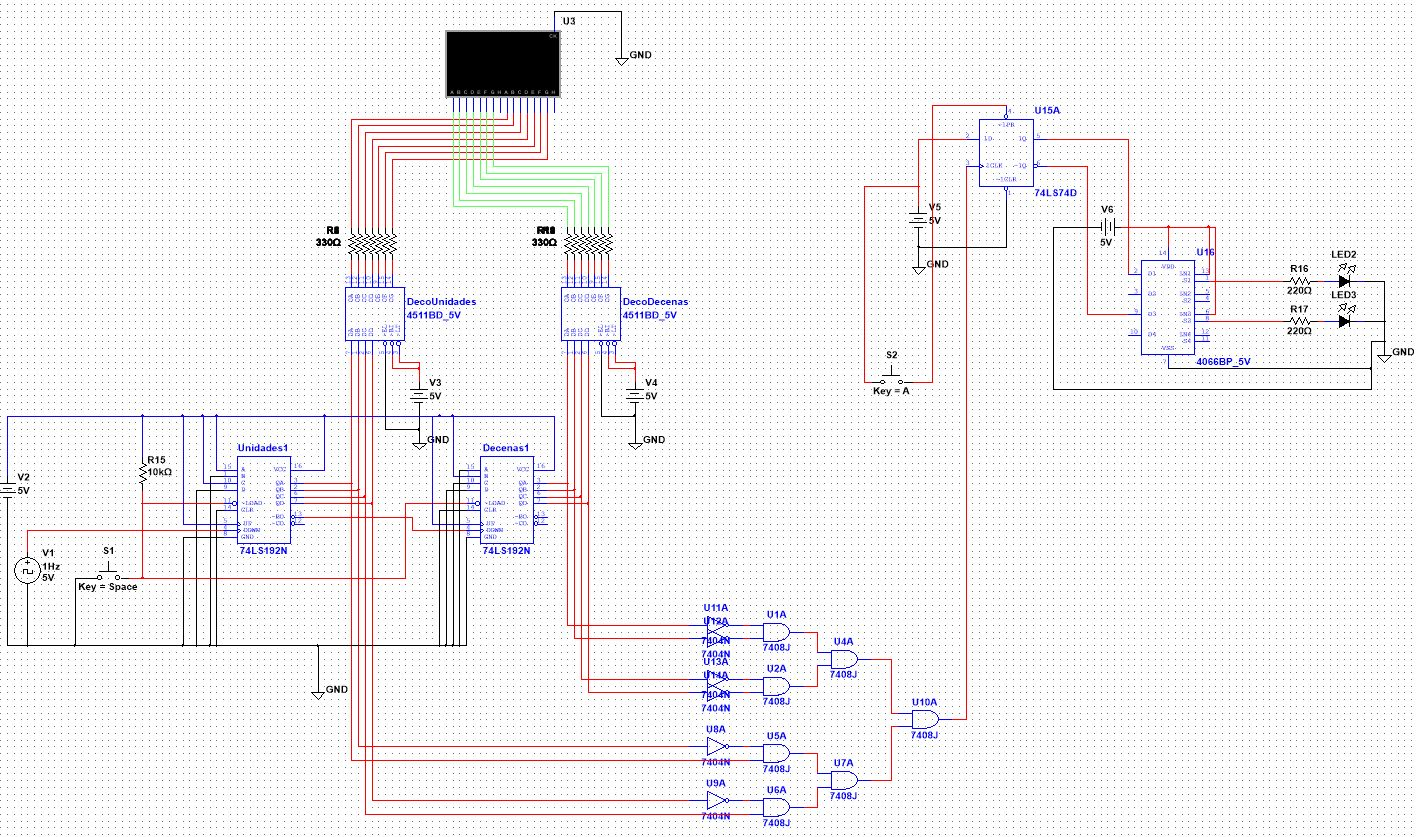
\includegraphics[width=0.85\columnwidth]{esquematico2}
\caption{Esquematico del subsistema de control: display de 7 segmentos, contadores y buzzer.}
\label{fig:proto_7seg}
\end{figure}

\begin{figure}[H]
\centering
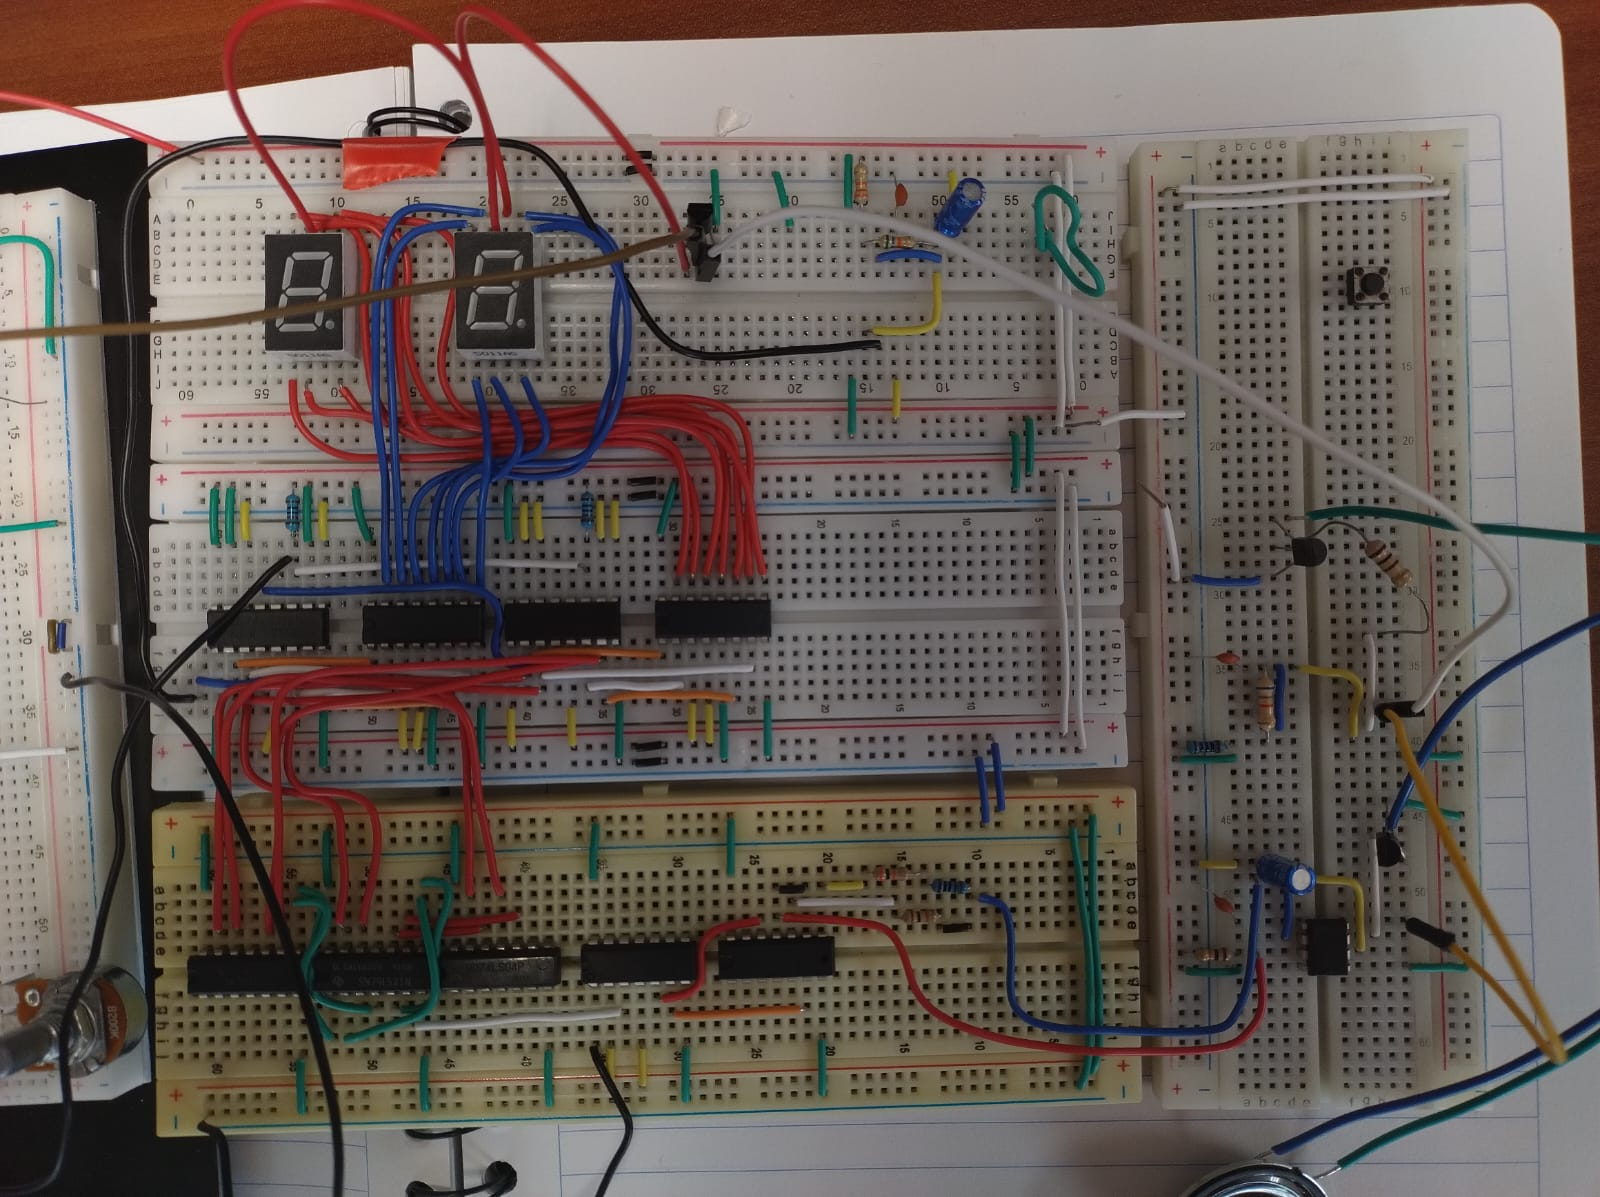
\includegraphics[width=0.85\columnwidth]{7segmentos1}
\caption{Prototipo en protoboard del subsistema de control: display de 7 segmentos, contadores y buzzer.}
\label{fig:proto_7seg}
\end{figure}

% ----------------------------------------------------------
\subsection{Subsistema 3: Iluminación (LED Vehicular y Peatonal)}
\label{subsec:leds}

Este subsistema se encarga de encender y apagar los arreglos de LEDs correspondientes a las luces vehiculares (rojo, amarillo y verde) y peatonales (rojo y verde), según las señales de control generadas por la máquina de estados.

\subsubsection{Descripción del circuito implementado}

La conmutación de los LEDs se controla mediante señales lógicas provenientes del subsistema de control. Se utilizó el temporizador dual NE556 junto con compuertas lógicas 74LS02 (NOR cuádruple) y 74LS05 (inversor hexagonal con salida en colector abierto) para generar y acondicionar las señales de activación de cada color. Todos los LEDs vehiculares y peatonales son manejados por transistores 2N2222A en configuración de conmutación. Los componentes principales son resistencias de \SI{330}{\ohm} para limitar la corriente en cada LED, resistencias variables de \SI{10}{\kilo\ohm} y \SI{50}{\kilo\ohm} junto con capacitores de \SI{100}{\micro\farad} y \SI{10}{\nano\farad} para ajuste de tiempos, y un diodo 1N4001 para protección en algunas ramas.

\subsubsection{Cálculo de resistencia limitadora}

La resistencia en serie con cada LED se calcula con:

\begin{equation}
R_{LED} = \frac{V_{CC} - V_F}{I_F}
\end{equation}

Con $V_{CC} = \SI{5}{\volt}$, $V_F \approx \SI{2}{\volt}$ (LED rojo/amarillo) e $I_F \approx \SI{10}{\milli\ampere}$, se obtiene $R_{LED} = \SI{300}{\ohm}$, por lo que se selecciona el valor estándar de \SI{330}{\ohm}, el cual garantiza brillo adecuado sin exceder la corriente máxima de los LEDs ni de las salidas TTL.

\subsubsection{Control lógico de las luces}

Las señales de habilitación para cada color provienen de la máquina de estados y son procesadas mediante las compuertas 74LS02 y 74LS05. La salida en colector abierto del 74LS05 facilita el acople directo a los transistores driver sin etapas adicionales de adaptación. El temporizador NE556 genera las secuencias temporizadas complementarias a la lógica principal. La Fig.~\ref{fig:leds_logica} muestra la interconexión simplificada de este subsistema.

\begin{figure}[H]
\centering
\resizebox{0.92\columnwidth}{!}{%
\begin{tikzpicture}[
    block/.style={draw, rectangle, rounded corners, minimum width=1.7cm, minimum height=0.8cm, align=center, font=\scriptsize},
    arrow/.style={-{Latex[length=1.6mm]}, thick}
]

% --- Fila superior: cascada de osciladores ---
\node[block] (ic1) at (0,0) {NE566};
\node[block] (ic2) at (4.4,0) {NE556\\\#1};
\node[block] (ic3) at (8.8,0) {NE556\\\#2};

% --- Periféricos asociados a cada oscilador ---
\node[block] (boton) at (-2.2,-1.5) {Botón};
\node[block] (ledr1) at (0,-1.5) {LED rojo};
\node[block] (diodo) at (4.4,-1.5) {1N4001};
\node[block] (leda) at (8.8,-1.5) {LED\\amarillo};

% --- Arreglo de compuertas ---
\node[block] (g1) at (4.4,-3.0) {74LS02};
\node[block] (g2) at (7.0,-4.5) {74LS05};

% --- Salidas hacia indicadores ---
\node[block] (ledv1) at (2.3,-4.5) {LED\\verde};
\node[block] (ledr2) at (4.4,-4.5) {LED\\rojo};
\node[block] (ledv2) at (7.0,-6.0) {LED\\verde};

% --- Conexiones: cascada de temporizadores ---
\draw[arrow] (boton) -- (ic1);
\draw[arrow] (ic1) -- (ledr1);
\draw[arrow] (ic1) -- (ic2) node[midway, above, font=\tiny]{señal};
\draw[arrow] (ic2) -- (diodo);
\draw[arrow] (ic2) -- (ic3) node[midway, above, font=\tiny]{señal};
\draw[arrow] (ic3) -- (leda);

% --- Conexiones: lógica de combinación ---
\draw[arrow] (ic1) -- (g1) node[midway, left, font=\tiny]{señal 1};
\draw[arrow] (ic3) -- (g1) node[midway, right, font=\tiny]{señal ppal.};
\draw[arrow] (g1) -- (ledv1);
\draw[arrow] (g1) -- (ledr2);
\draw[arrow] (g1) -- (g2);
\draw[arrow] (g2) -- (ledv2);

\end{tikzpicture}}
\caption{Interconexión simplificada del subsistema de iluminación: cascada de osciladores NE566/NE556 y lógica de combinación mediante compuertas 74LS02/74LS05 hacia los LEDs vehiculares y peatonales.}
\label{fig:leds_logica}
\end{figure}

\subsubsection{Prototipo del subsistema de iluminación}

La Fig.~\ref{fig:proto_leds} muestra la protoboard correspondiente al subsistema de iluminación y control de fases semafóricas. Los circuitos integrados presentes en esta etapa incluyen los temporizadores LM555 o NE556 como generadores de las bases de tiempo para cada fase del ciclo, los inversores 7404N y las compuertas AND 7408J que conforman la lógica combinacional de habilitación de cada color, y los transistores 2N2222A como drivers de conmutación para los arreglos de LEDs vehiculares y peatonales. Parte de estos componentes fue solicitada en la bodega del laboratorio y el resto adquirido por el equipo, obteniéndose en todos los casos integrados de distintos fabricantes pero con pinout y especificaciones eléctricas equivalentes. El cableado, realizado con cables de protoboard estándar, resultó en un arreglo funcional aunque con cierta densidad visual dada la cantidad de interconexiones entre integrados.
\begin{figure}[H]
\centering
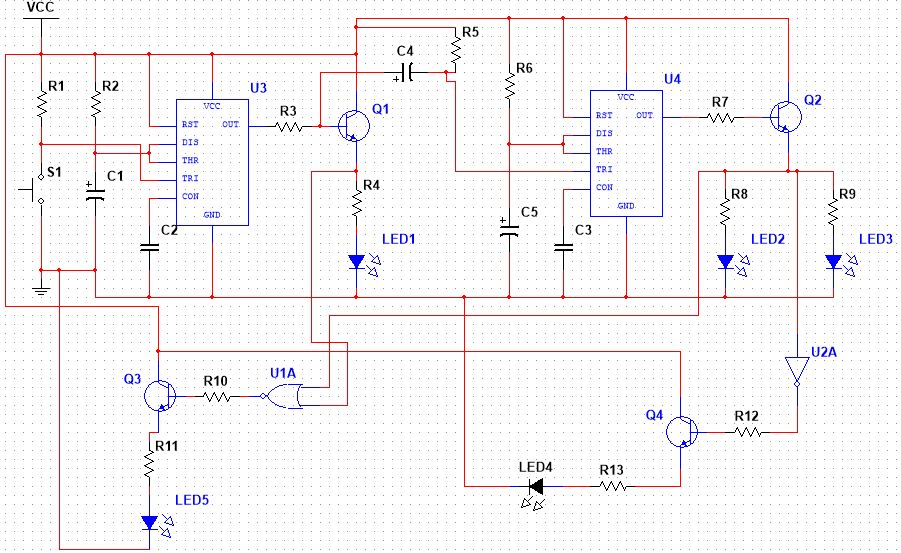
\includegraphics[width=0.85\columnwidth]{esquematicoleds1}
\caption{Esquematico del subsistema de luces del semaforo: LEDs vehiculares y peatonales con su lógica de control.}
\label{fig:proto_leds}
\end{figure}


\begin{figure}[H]
\centering
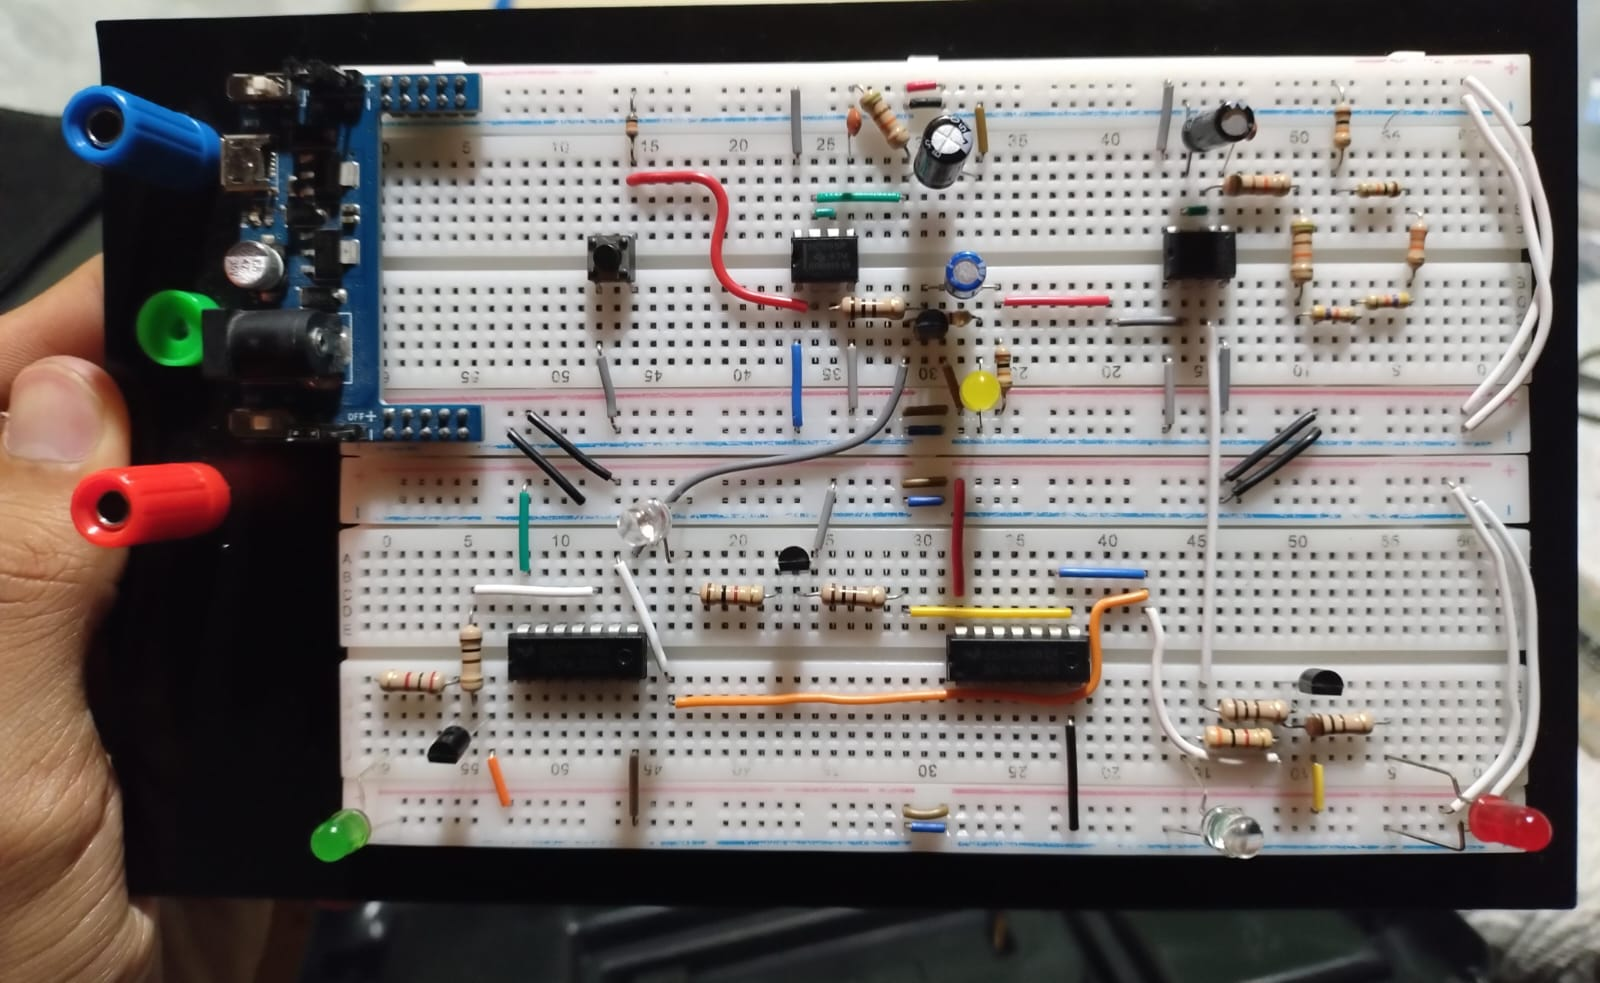
\includegraphics[width=0.85\columnwidth]{leds1}
\caption{Prototipo en protoboard del subsistema de iluminación: LEDs vehiculares y peatonales con su lógica de control.}
\label{fig:proto_leds}
\end{figure}

\subsubsection{Consideraciones de diseño y potencia en PCB}

Para la implementación física en PCB se deberá evaluar la necesidad de etapas de potencia adicionales según la cantidad de LEDs por color. Los conductores que transportan la corriente de los arreglos de LED deben dimensionarse conforme a las curvas estándar de IPC-2221, evitando rutas largas y estrechas que concentren disipación resistiva ($P = I^2 R_{pista}$) en zonas críticas. Si el zumbador es electromecánico, se recomienda incluir un diodo de libre circulación en paralelo para proteger los transistores driver contra transitorios inductivos.

% ----------------------------------------------------------
\subsection{Maqueta física del sistema}
\label{subsec:maqueta}

La maqueta se construyó con forma rectangular, integrando los postes de semáforo vehicular y peatonal junto con la representación de la vía. Las Figs.11 y 12 muestran la maqueta desde una vista horizontal general y una vista frontal respectivamente. Debido a las restricciones de tiempo del proyecto y a las dimensiones físicas de los componentes disponibles —en particular los displays de 7 segmentos y los arreglos de LEDs montados sobre los postes—, la maqueta presenta una desproporción notable entre el tamaño de los elementos electrónicos y la escala de la calle simulada, resultando en un espacio reducido entre los postes y en una apariencia en la que los componentes dominan visualmente sobre la representación de la vía. Este aspecto constituye un punto de mejora identificado para versiones futuras del prototipo.

\begin{figure}[H]
\centering
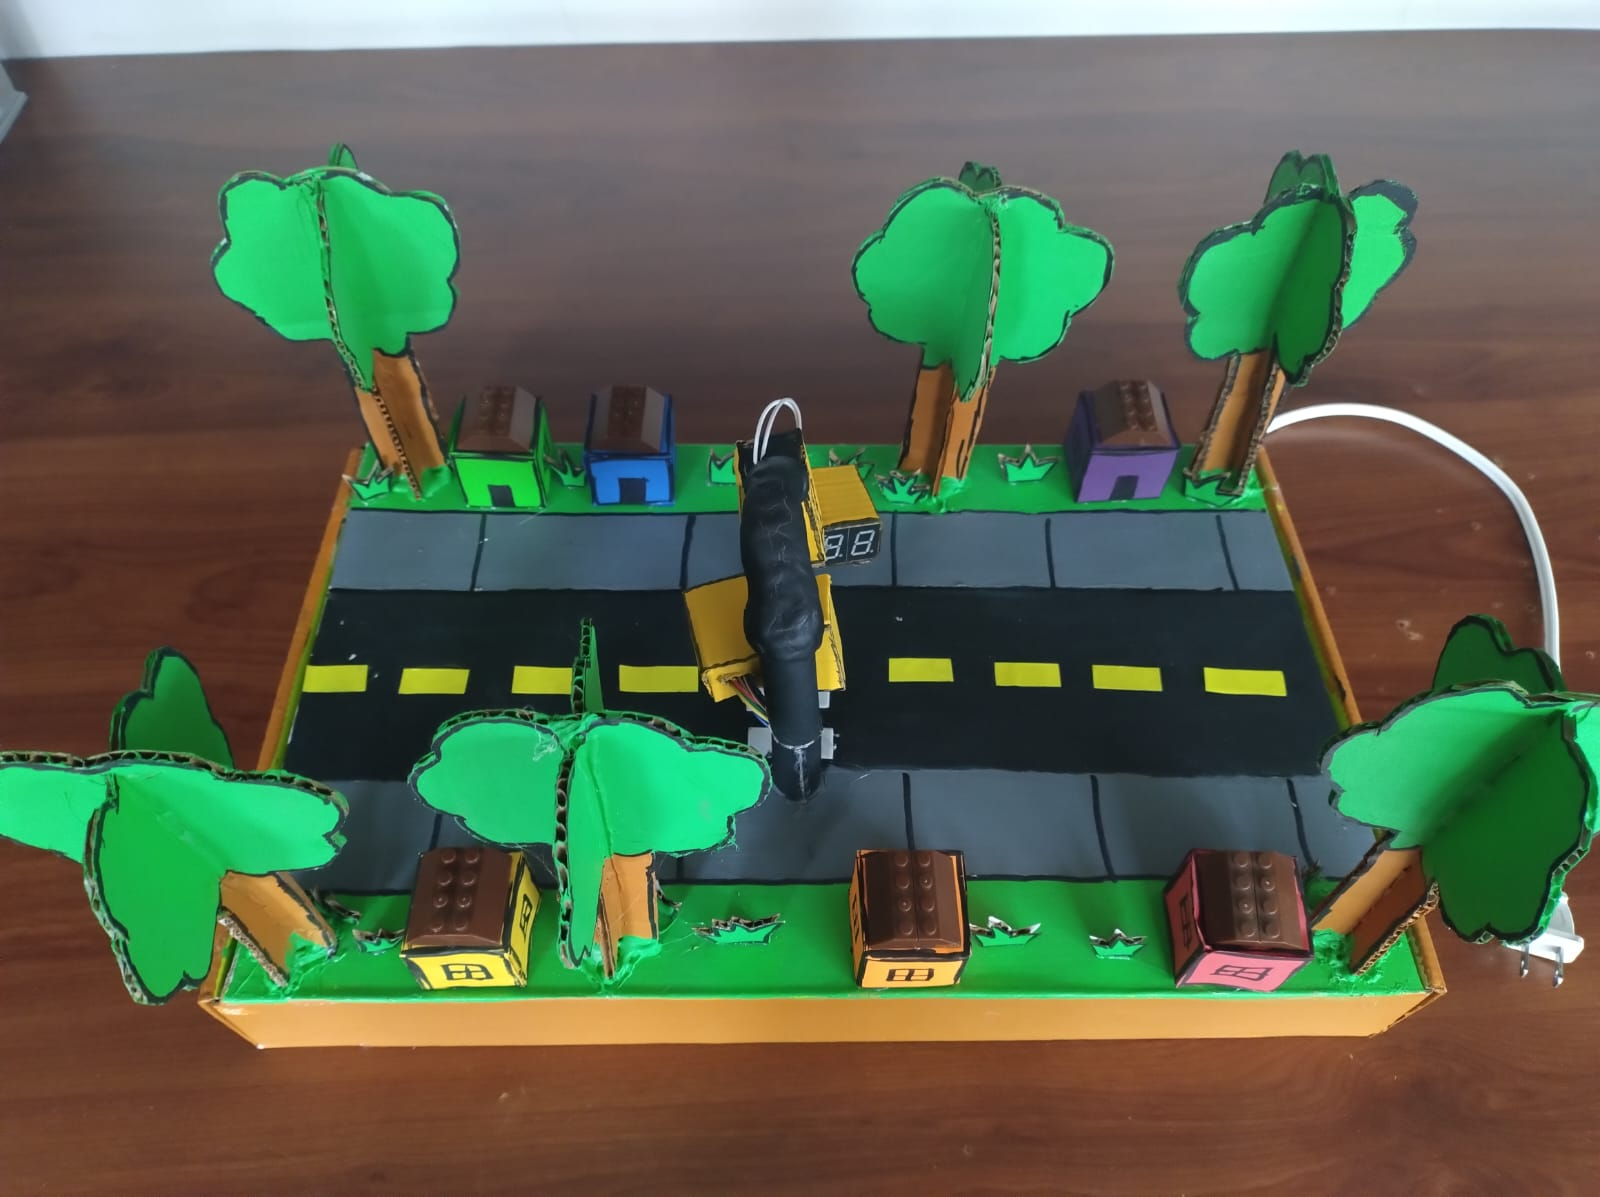
\includegraphics[width=0.85\columnwidth]{maqueta1}
\caption{Vista horizontal general de la maqueta del sistema semafórico.}
\label{fig:maqueta_horizontal}
\end{figure}

\begin{figure}[H]
\centering
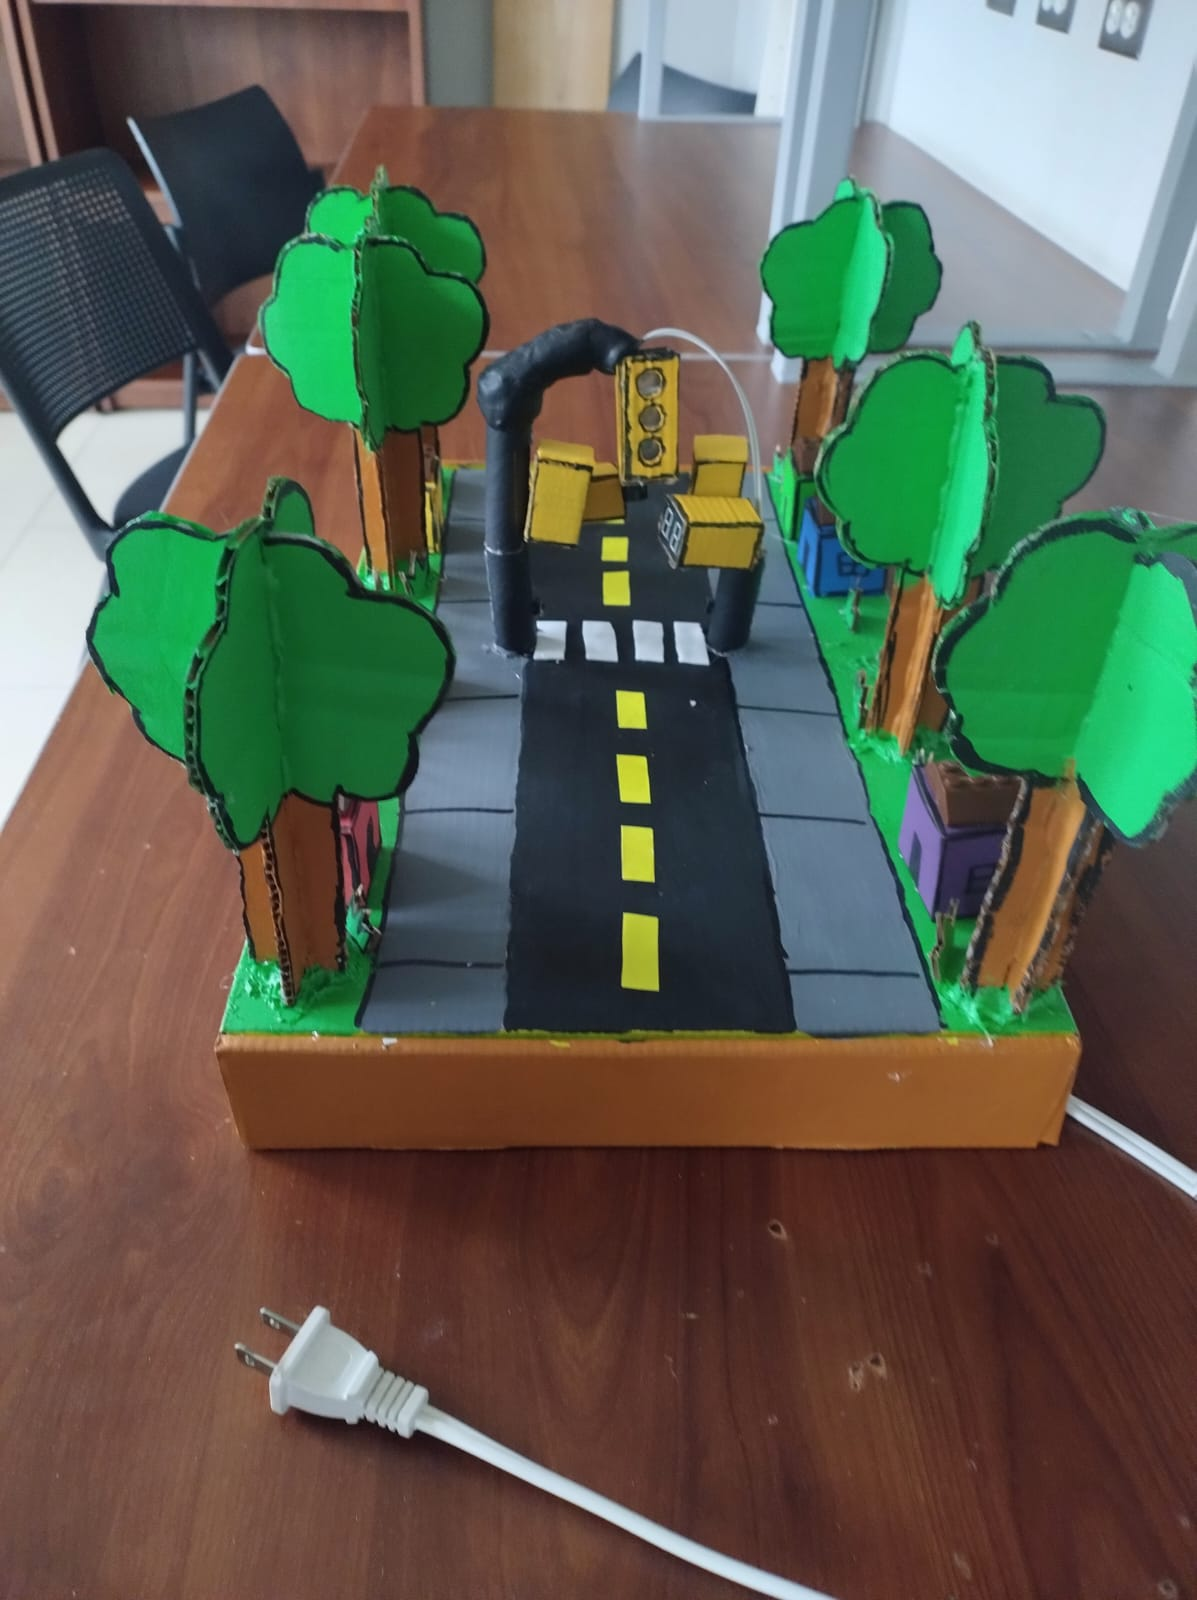
\includegraphics[width=0.85\columnwidth]{maqueta2}
\caption{Vista frontal de la maqueta del sistema semafórico.}
\label{fig:maqueta_frontal}
\end{figure}


% 5. SECUENCIA DE OPERACIÓN

\section{Secuencia de Operación}
\label{sec:operacion}

Al arrancar, los contadores se cargan con el valor 25 gracias a los preajustes y al pulso inicial en el pin LOAD (generado por el circuito RC asociado al nodo de reset). El verde vehicular y el rojo peatonal se encienden, y la cuenta regresiva inicia desde 25.

Cuando la cuenta llega a 0, la lógica combinacional (NOR de decenas más arreglo AND de unidades) genera un flanco en 1CLK del 74LS74, que conmuta las salidas 1Q y $\overline{1Q}$. Este cambio activa el DPDT y, mediante el nodo de RST de los temporizadores, apaga el verde vehicular y enciende el amarillo durante aproximadamente 3 segundos. Tras este intervalo, el Temporizador 2 toma el control: apaga el amarillo, enciende el rojo vehicular y el verde peatonal, y apaga el rojo peatonal. Durante esta fase los temporizadores de sonido activan el buzzer de forma intermitente. El ciclo se repite automáticamente o puede ser solicitado en cualquier momento con el botón peatonal.


% 6. CRITERIOS DE SELECCIÓN DE COMPONENTES

\section{Criterios de Selección de Componentes}

La implementación se realizó principalmente con la familia lógica TTL (serie 74LS y 74xx) por su disponibilidad en el laboratorio y buena capacidad de fan-out para excitar displays y LEDs indicadores. La Tabla~\ref{tab:componentes} resume los criterios de selección de los componentes principales.

\begin{table}[H]
\centering
\caption{Criterios de selección de componentes principales}
\label{tab:componentes}
\begin{tabular}{>{\bfseries}p{2.5cm} p{5.5cm}}
\toprule
Componente & Criterio de selección \\
\midrule
LM555 & Bajo costo, rango de alimentación amplio (4.5--16 V), capacidad de excitar hasta 200 mA, fácil configuración astable/monostable. \\
74LS192N & Contador BCD síncrono con precarga asíncrona; salida Borrow facilita cascada para dos dígitos. \\
4511BD & Decodificador BCD a 7 segmentos con salidas de alta corriente para display de cátodo común, con entradas de blanking y test. \\
LM7805 & Regulador de tensión fijo de 5 V con protección térmica y de cortocircuito, ideal para lógica TTL/CMOS. \\
1N4007 & Diodo rectificador de propósito general, 1 A / 1000 V, amplio margen de seguridad en arranque. \\
2N2222A & Transistor NPN de baja potencia, alta ganancia y conmutación rápida; manejo de LEDs y buzzer. \\
74LS74D & Flip-flop tipo D con precarga y clear; sincroniza eventos y mantiene estados con bajo consumo. \\
7408J / 7404N / 74ALS02 & Compuertas lógicas TTL estándar de bajo consumo, compatibles con niveles de +5 V. \\
NE556 & Doble temporizador 555 en un solo encapsulado; reduce cantidad de componentes frente a usar cuatro 555 individuales. \\
74LS02 / 74LS05 & NOR cuádruple e inversor con salida en colector abierto; combinan e invierten señales de los temporizadores para la secuencia de LEDs. \\
\bottomrule
\end{tabular}
\end{table}

La mezcla de familias TTL y CMOS (4511BD) fue posible porque ambas operan correctamente a \SI{5}{\volt}. La serie 74LS se eligió sobre la serie 4000 por su menor tiempo de propagación y mayor capacidad de corriente de salida, aunque para este proyecto —donde las bases de tiempo son del orden de \SI{1}{\hertz}— la velocidad de conmutación no es un factor crítico. La salida en colector abierto del 74LS05 facilita acoplar directamente LEDs sin etapas adicionales de adaptación de corriente. El diodo 1N4001 en el subsistema de iluminación protege nodos sensibles con suficiente margen (\SI{50}{\volt} inversos, \SI{1}{\ampere}) sin sobredimensionar como en la etapa de rectificación principal.


% 7. SIMULACIÓN

\section{Simulación}

La validación funcional del diseño se realizó en el simulador Multisim siguiendo una estrategia de integración incremental por subsistemas.

\subsection{Resultados del subsistema de alimentación}

\begin{itemize}
    \item Salida del transformador (secundario): \SI{12}{\volt_{AC}} (valor nominal).
    \item Después del puente rectificador y capacitor de filtro (\SI{4700}{\micro\farad}): voltaje DC promedio = \SI{15.918}{\volt}, rizado = \SI{100.775}{\milli\volt_{pp}}.
    \item Salida del regulador LM7805: voltaje DC = \SI{5}{\volt} (estable y regulado), rizado = \SI{18.448}{\micro\volt_{pp}}.
\end{itemize}

Con la resistencia de carga de \SI{50}{\ohm}:

\[
I_L = \frac{5}{50} = \SI{100}{\milli\ampere}, \qquad P_D = (15.918 - 5) \times 0.1 \approx \SI{1.09}{\watt}
\]

Estos resultados confirman un excelente desempeño: el rizado a la salida del regulador es prácticamente negligible (\SI{18.45}{\micro\volt}), garantizando alimentación limpia para la lógica digital, y la disipación térmica de \SI{1.09}{\watt} es manejable con el disipador instalado.

\subsection{Plan de integración incremental}

\begin{enumerate}
    \item Simulación aislada de la fuente de alimentación: verificación de voltaje, rizado y regulación del LM7805 bajo variación de carga.
    \item Simulación del bloque de control: osciladores 555, contadores 74LS192, decodificadores 4511 y máquina de estados con 74LS74.
    \item Simulación del generador de audio y amplificador con 2N2222A, verificando la conmutación de frecuencia al detectar el valor 5 en la cuenta regresiva.
    \item Integración completa de los tres subsistemas, verificando la secuencia de luces, la cuenta regresiva en el display y la señal sonora; se comprueba además que no exista caída de tensión significativa en los rieles de alimentación al conmutar simultáneamente todos los arreglos de LED.
\end{enumerate}


% 8. CONSIDERACIONES PARA EL PCB

\section{Consideraciones para el PCB}

La implementación física se distribuirá en al menos dos placas de circuito impreso:

\begin{itemize}
    \item \textbf{PCB 1}: Subsistema de alimentación completo (rectificador, filtro capacitivo, regulador LM7805 con disipador).
\end{itemize}
 Por tiempo, orden y simplificar, se decidio utilizar la fuente de alimentación para el diseño e impresion en PCB

% REFERENCIAS

\begin{thebibliography}{99}

\bibitem{boylestad} R. L. Boylestad y L. Nashelsky, \emph{Electrónica: Teoría de Circuitos y Dispositivos Electrónicos}, 11.\textsuperscript{a} ed. Ciudad de México, México: Pearson Educación, 2013.

\bibitem{floyd} T. L. Floyd, \emph{Fundamentos de Sistemas Digitales}, 11.\textsuperscript{a} ed. Madrid, España: Pearson Educación, 2015.

\bibitem{sedra} A. S. Sedra y K. C. Smith, \emph{Microelectronic Circuits}, 7.\textsuperscript{a} ed. New York, NY, USA: Oxford University Press, 2014.

\bibitem{lm555} Texas Instruments, \emph{LM555 Timer}, Datasheet SNOSBCH2D, revisado mayo 2015. [En línea]. Disponible: \url{https://www.ti.com/lit/ds/symlink/lm555.pdf}

\bibitem{ls192} Texas Instruments, \emph{SN54LS192, SN74LS192 Synchronous 4-Bit Up/Down Counters (Dual Clock With Clear)}, Datasheet SDLS074, diciembre 1972, revisado marzo 1988. [En línea]. Disponible: \url{https://www.ti.com/product/SN74LS192}

\bibitem{cd4511} Texas Instruments, \emph{CD4511B CMOS BCD-to-7-Segment Latch/Decoder/Driver}, Datasheet SCHS072B, adquirido de Harris Semiconductor, revisado julio 2003. [En línea]. Disponible: \url{https://www.ti.com/lit/ds/symlink/cd4511b.pdf}

\bibitem{lm7805} Texas Instruments, \emph{LM340, LM340A and LM7805 Family Wide VIN 1.5-A Fixed Voltage Regulators}, Datasheet SNOSBT0L, febrero 2000, revisado septiembre 2016. [En línea]. Disponible: \url{https://www.ti.com/lit/ds/symlink/lm340.pdf}

\bibitem{ls74a} Texas Instruments, \emph{SN54LS74A, SN74LS74A Dual D-Type Positive-Edge-Triggered Flip-Flops with Preset and Clear}, Datasheet SDLS119, diciembre 1983, revisado marzo 1988. [En línea]. Disponible: \url{https://www.ti.com/lit/ds/symlink/sn74ls74a.pdf}

\bibitem{7404} Texas Instruments, \emph{SN54LS04, SN74LS04 Hex Inverters}, Datasheet SDLS025, revisado marzo 1988. [En línea]. Disponible: \url{https://www.ti.com/product/SN74LS04}

\bibitem{7408} Texas Instruments, \emph{SN54LS08, SN74LS08 Quadruple 2-Input AND Gates}, Datasheet SDLS033, revisado marzo 1988. [En línea]. Disponible: \url{https://www.ti.com/product/SN74LS08}

\bibitem{74ls02} Texas Instruments, \emph{SN54LS02, SN74LS02 Quadruple 2-Input NOR Gates}, Datasheet SDLS001, revisado marzo 1988. [En línea]. Disponible: \url{https://www.ti.com/product/SN74LS02}

\bibitem{ne556} Texas Instruments, \emph{NE556, SA556, SE556 Dual Timer}, Datasheet SLAS568A, revisado 2008. [En línea]. Disponible: \url{https://www.ti.com/product/NE556}

\bibitem{2n2222a} ON Semiconductor (onsemi), \emph{2N2222A Small Signal Switching Transistor, NPN Silicon}, Datasheet 2N2222A/D, noviembre 2013, Rev.~2. [En línea]. Disponible: \url{https://www.onsemi.com/download/data-sheet/pdf/2n2222a-d.pdf}

\bibitem{1n4007} ON Semiconductor (onsemi), \emph{1N4001--1N4007 Axial-Lead Glass Passivated Standard Recovery Rectifiers}, Datasheet 1N4001/D, junio 2024, Rev.~18. [En línea]. Disponible: \url{https://www.onsemi.com/download/data-sheet/pdf/1n4001-d.pdf}

\bibitem{ipc2221} IPC, \emph{IPC-2221B: Generic Standard on Printed Board Design}, Bannockburn, IL, USA: IPC, 2012.

\end{thebibliography}

\end{document}